\section{virtual\_evolution} \label{sec-virtual-ev}

The tools \emph{virtual\_evolution} and
\emph{virtual\_evolution\_controlled} allow you to simulate simple
evolutionary processes and create nucleic sequences ressembling to
evolutionary processes. Your simulated biosphere shall hence
reside in a FASTA file.

\subsection{Usage}

The evolution simulation as implemented
in MNHN-Tree-Tools comes in two versions: A rather crude
\emph{virtual\_evolution} tool and in a more controlled, later
added \emph{virtual\_evolution\_controlled} tool.

The tools can be called as outlined in the following:

The \emph{tree\_map\_for\_sequence} tool can be used:
\lstset{language=bash,
  caption={Calling the \emph{virtual\_evolution} tools},
  label=lst-virtev-call}
\begin{lstlisting}
virtual_evolution [seed] [seq-length] [n-sequences] [n-partitions] \
  [max-time] [rate] [n-mutations-to-amplification-template] [fasta]
virtual_evolution_controlled [seed] [seq-length] [n-sequences] [n-partitions] \
  [max-time] [rate] [n-mutations-to-previous-amplification-template] [fasta]
\end{lstlisting}
with the parameters:
\begin{enumerate}
  \item \emph{seed} The seed the pseudorandom number generator uses.
    This value allows us to generate the same set of sequences
    in subsequent calls of this tool.
  \item \emph{seq-length} The length of the sequences to be generated.
  \item \emph{n-sequences} How many sequences in total have to be
    generated.
  \item \emph{n-partitions} How many families/clusters shall be
    generated, or in other words, how many amplification events should happen.
  \item \emph{max-time} This value selects if the evolution should
    occur at random times beteween amplifications and be limited to
    \emph{max-time} or weather, if -1 is chosen 
    a constant evolution cycle befor a new cluster expansion
    happens is prefered. If the value selected is not -1  a random
    number, between 0 and \emph{max-time} of evolution cycles may occur.
  \item \emph{rate} The substitution rate of nucleotide
    bases in the nucleic sequences per evolution cycle.
  \item \emph{n-mutations-to-amplication-template} Adds the here
    chosen number of mutation to the amplification template before a
    new cluster expansion occurs.
    In this case the nucleotide bases are only replaced $X$
    times, as chosen here. The actual number of mutations
    might be lower as the replaced bases (at a probablity of 1/4th per
    base) might be of the same nucleotide as the one that was in place.
  \item \emph{n-mutations-to-previous-amplification-template} Adds
    this number of real mutations to the previous amplification
    template, before generating a new family.
  \item \emph{fasta} A FASTA file where to write the sequences
    generated to.
\end{enumerate}

\subsection{Algorithm}
As the algorithms for the two simulation processes are different we
outline both in the following:
\begin{itemize}
  \item \emph{virtual\_evolution} process. The evolutionary process
    herein is a basic expansion and diffusion process. The way this
    simulator works is that it generates a template sequence of a
    given size. It then copies this template sequence until it fills a whole
    family as defined by the \emph{n-sequences} and
    \emph{n-partitions} arguments. A family or partition as such
    contains
    \begin{equation}
      N = n_{\mathrm{seq}}/n_{\mathrm{part}},
    \end{equation} sequences where
    $n_{\mathrm{seq}}$ are the number of total sequences and
    $n_{\mathrm{part}}$ are the number of partitions or families to be
    created. It than performs
    \begin{equation}
      M = ptr \label{eqn-mutation-rate}
    \end{equation}
    mutations on the previous partitions generated. Where $t$ is a random
    time, and hence the number of cycles number, which is chosen between 0
    and $t_{\mathrm{max}}$ which is defined by the \emph{max-time}
    parameter. $r$ is the mutation rate as defined by the \emph{rate}
    parameter. $p$ is the number of partitions already generated.
    Once $M$ mutation were perfomed on the current state of the
    dataset a sequence randomly chosen from the previous
    sequencies will be the template for the next expension of $N$
    sequences. The algorithm is continued until all partitions are
    created, perfoming a last mutation run on the entire dataset as
    determined by equation \ref{eqn-mutation-rate}.
    The whole process is further outlined in figure
    \ref{fig-virtual-evolution}.
  \item \emph{virtual\_evolution\_controlled} is a different, simpler
    but more controlable process. The main difference to the
    uncontrolled \emph{virtual\_evolution\_process} is that the
    template for each family is chosen from the previous template to
    create a partition or family, and not randomly chosen from the
    existing sequences. Further the number of mutations is enforced
    not be just exchanges of nucleotides, that might actually not lead
    to mutations as there is a 1 in 4 chance that a nucleotide gets
    replaced by itself, but to be actual mutations. Hence, one
    perfectly knows to what extend the templates between families
    differ. Together with a
    fixed mutation rate one can further perfectly estimate the diffusion of
    each partition. As such we have created a perfectly controlled
    distance-diffusion mechanism. The process is outlined in figure
    \ref{fig-virtual-evolution-controlled}.
\end{itemize}
\begin{figure}
  \begin{center}
  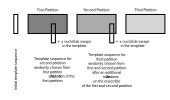
\includegraphics[scale=0.9]{virtual-evolution.pdf}
  \caption{The classic virtual evolution process. The different levels of gray
    show how diffused, (old) the sequences are at the end of the
    process. Please note that $t$ is chosen at random after each
    partition expension.}
  \label{fig-virtual-evolution}
  \end{center}
\end{figure}
\begin{figure}
  \begin{center}
  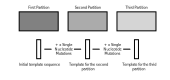
\includegraphics[scale=0.9]{virtual-evolution-controlled.pdf}
  \caption{The more restricted controlled virtual evolution
    process. The different level of gray show how diffused, (old) the
    sequences are at the end of the process. Again note there are
    $M = ptr$ mutations happening across the available sequences after
    each expansion and that $t$ might be variable if chosen so.}
  \label{fig-virtual-evolution-controlled}
  \end{center}
\end{figure}

\subsection{Example}
\lstset{language=bash,
  caption={An example of how to use the \emph{virtual\_evolution} tools.},
  label=lst-virtev-example}
\begin{lstlisting}
virtual_evolution_controlled 42 100 10000 10 -1 1000 4 biosphere.fasta
\end{lstlisting}
In this example the evolutionary process generates 10000 sequences of 100
nucleotides, in 10 partitions of 1000 sequences and a mutation rate
$r=1000$. The time $t=1$, or number of cycles is fixed to one in order
for the diffusion to stay constant during the process. The template
undergoes 4 mutations before creating each new family. The resulting
sequences are stored to \emph{biosphere.fasta}.

\subsection{Implementation}
\emph{virtual\_evolution} and \emph{virtual\_evolution\_controlled}
are implemented in \emph{virtual\_evolution.c} and
\emph{virtual\_evolution\_controlled.c} respectivly. 




